\chapter{A Cell Is Not a Little Bag of Liquid}

\begin{kaichang}
Take a raw egg from the kitchen, crack it, and pour the white and intact yolk into a bowl. The round yolk is enclosed in an almost invisible membrane. Gently poke it with a chopstick: the membrane breaks and thick yellow liquid flows out.

\textbf{Translator safety note:} Do not taste the raw egg. Wash hands, utensils, and the work surface after handling it, and keep it separate from ready-to-eat food. See \href{https://www.fda.gov/food/retail-food-industryregulatory-assistance-training/assuring-safety-eggs-and-menu-and-deli-items-made-raw-shell-eggs}{FDA raw-egg safety guidance}.

Here is an unusual fact: biologically, that yolk counts as \emph{one cell}. The yolk membrane enclosing it is its cell membrane. A chicken yolk is about three centimeters across; an ostrich yolk can be fist-sized. They are among Earth's largest individual cells.

Now guess: is the yellow liquid simply cell fluid? Is a cell just a little bag of nutrient soup, with organelles floating like dumplings? Many people first picture cells this way, reinforced by textbook illustrations: a circle containing a few floating colored parts. Write down your answer. At the end, we return to the yolk and discover that a real cell interior is far more extraordinary than a bag of soup.
\end{kaichang}

\section{Under the Microscope: Cells Are Never Empty}

Begin with what can be seen. An onion-epidermis wet mount under a microscope shows bricklike compartments, each with a darker dot, the nucleus. Switch to a drop of pond water and the scene becomes a busy street: paramecia race past, diatoms drift like glass boats, and particles visibly move inside some cells.

An aquatic plant called Hydrilla is especially revealing. In a young leaf, green chloroplasts circulate in lines around each cell's inner wall like a ring conveyor belt. This is \textbf{cytoplasmic streaming}. If cells were bags of motionless soup, that conveyor could not run: nothing in the soup would push chloroplasts in a particular direction.

A more familiar scene: after you scrape a finger, a scab forms and the wound heals over several days as skin cells divide, crawl, and fill the gap. Cells \emph{crawl}, change shape, and transport things from one end to another. A motionless liquid bag cannot. Visible light provides the first evidence: cells have internal structures, and those structures keep moving.

\section{Closer In: Thick Porridge, Not Clear Soup}

Magnify beyond optical limits into electron microscopy. The first shock is that \textbf{cells are extremely crowded}.

Some numbers help. One Escherichia coli bacterium, about \ud{2}{\mu m} long and small enough for billions potentially to live beneath your fingernail, contains roughly $3\times10^{6}$ protein molecules, thousands of ribosomes, a circular DNA molecule, and countless small molecules. Altogether, the macromolecules occupy about $30\%$ of its interior volume. What does $30\%$ mean? The fraction of a rush-hour subway carriage occupied by passengers is of a similar order. Your cells are larger and more crowded still.

Cytoplasm is thus not dilute soup but porridge almost too thick to stir. This matters because it shapes nearly everything a cell does. A protein moving through cytoplasm does not travel straight like a stone falling through water; it is more like you weaving through a holiday railway-station crowd, colliding and detouring with hundreds of others each step. Molecules have no private space. Crowds push enzymes and substrates together. As we will see, cells address crowding not by reducing population, but by building railways.

\section{Two Basic Layouts: Prokaryotic and Eukaryotic}

Earth's cells have two basic layouts with a clear distinction.

\textbf{Prokaryotic cells}, bacteria and archaea, lack nuclei. Their coiled DNA occupies a nucleoid region without a surrounding membrane. Apart from the cell membrane, internal membranes are nearly absent. Usually only one or two micrometers across, they accomplish most internal transport through random diffusion and need no elaborate compartments. But prokaryotic does not mean unorganized porridge: DNA has defined locations, proteins cluster by function, and dedicated protein supports maintain shape. They simply do without walled offices.

\textbf{Eukaryotic cells}, including yours, mushrooms, kelp, and paramecia, are much larger, typically $10$ to \ud{100}{\mu m} across. Membranes divide their interiors into rooms called \textbf{organelles}. Human, yeast, and onion cells share this layout. Chapter 56 said the earliest eukaryotic cells appeared around two billion years ago; this internal membrane system enabled larger, more complex cells.

Clarify one thing: a membrane is not merely a bag. It is a \textbf{working surface}. Chapter 51 explained that phospholipid bilayers block most charged substances, allowing different pH values and ion concentrations on opposite sides. The membrane itself is a dam capable of storing a gradient for power. Chapter 53's respiratory chain and Chapter 54's photosynthetic chain both work on membranes. Once membranes become workbenches, organelles cease to be a list of names.

\section{Tour the Rooms, but Look at the Machinery}

Textbooks call the nucleus a control center, mitochondria power stations, and the Golgi apparatus a post office, then ask you to memorize them. These analogies help with locations but say nothing about mechanisms. We will ask one question of each organelle: \textbf{what are its membrane and protein molecules doing?}

\subsection{The Nucleus: A Vault with Security Gates}

The nuclear envelope is double, perforated by \textbf{nuclear pores}. A pore is not merely a hole but a screening machine built from dozens of protein types. It admits only proteins carrying particular passage signals, amino-acid sequences. DNA is too large and never leaves the nucleus; to execute instructions, the cell makes RNA copies and sends them out. Volume III's Chapters 67--69 examine transcription and translation. Vault plus security gates solves a real problem: eukaryotic DNA can be thousands of times longer than bacterial DNA and must be separated from cytoplasmic chemical turmoil while maintaining two-way communication.

\subsection{ER and Golgi: Folding and Sorting Workshops}

The endoplasmic reticulum is a vast membrane labyrinth extending from the nuclear envelope. Folding supplies enormous working area in a small volume, the same geometry as folds inside your small intestine. Ribosome-covered regions are rough ER. Newly made proteins thread directly into its lumen for folding and quality control; failed folds are marked for destruction, recalling protein folding in Chapter 49. Ribosome-free smooth ER is a lipid workshop, producing materials for the cell membrane and organelle membranes.

How do products reach the next station? In \textbf{vesicles}. A patch of ER membrane bulges outward, pinches off as a cargo-filled bubble, travels to the Golgi, fuses membranes, and unloads. The Golgi is a stack of flattened membrane sacs, like plates. Cargo enters one end and leaves the other, receiving labels along the way, mainly added or trimmed sugar chains that supply destination addresses, as in Chapter 47's sugars. Labeled cargo enters new vesicles bound for the cell membrane, lysosomes, or outside.

Why do vesicles not deliver to the wrong address? Membrane proteins recognize one another. Matching proteins on vesicle and target membranes have complementary shapes, meshing like zipper teeth to pull membranes together and force fusion. Unmatched membranes cannot join. Cellular logistics has no driver or map, only molecular locks and keys: Chapter 48's structure-determines-function principle on a grand scale.

\subsection{Lysosomes: Recycling with an Acid Safety Lock}

Lysosomes contain dozens of hydrolases that break down proteins, lipids, and sugars. An obvious danger is self-digestion if they leak. The chemical solution is proton pumps in the lysosomal membrane, continually spending ATP to pump \chem{H^+} inside and maintain an acidic $pH$ around $5$. These enzymes work at full strength only in acid and largely shut down in neutral cytoplasm. Acidity is one safeguard, neutral cytoplasm another. No intelligence is involved, only precise use of Chapter 34's relationship between $pH$ and enzyme activity. Lysosomes recycle aged organelles and digest engulfed bacteria. In lysosomal storage diseases, a defective hydrolase leaves material accumulating inside cells. Failure of a single enzyme can be fatal.

\subsection{Mitochondria and Chloroplasts: Energy Departments with IDs}

Chapters 53 and 54 explained their machinery: respiration converts electron-transfer energy into a membrane proton gradient, whose return flow rotates ATP synthase; photosynthesis uses light for a similar energy lift. Here, emphasize three features absent from other organelles: both have \emph{double} membranes, their own DNA and ribosomes for making a few proteins, and reproduction by division. A cell cannot make a mitochondrion from scratch; one grows only from an existing mitochondrion.

Why should an organelle need DNA of its own? These three peculiarities point to a remarkable story, saved for the evidence section.

\subsection{The Cytoskeleton: Rebuildable Scaffolds and Railways}

All these shapes and movements depend on a cell-spanning network of protein fibers called the \textbf{cytoskeleton}. It has two main track materials. Microtubules are hollow tubes about \ud{25}{nm} across, assembled from protein subunits placed end to end. Thinner microfilaments are chains of actin. Notice assembled: these tracks are \emph{alive}, adding parts at one end and removing them at the other every second. A new route can be laid in minutes when needed and dismantled afterward.

\textbf{Molecular motors} run on the tracks. One thoroughly studied motor, kinesin, alternates two feet along a microtubule, consuming one ATP per step. Hydrolysis sharply changes its shape, producing a step, as Chapter 50 explained. Its stride is about \ud{8}{nm}, with tens to hundreds of steps per second, carrying vesicles tens of times larger than itself. Part of what lets you think right now is kinesin hauling vesicles along meter-long microtubules from nerve-cell bodies to nerve endings.

Microfilaments provide the muscle: actin and myosin slide against each other to contract cells, enable crawling, and constrict dividing cells into two. Hydrilla's chloroplast conveyor is powered by microfilament tracks laid along the cell wall.

\section{Why Not Rely on Diffusion?}

\begin{qiaoliang}
Could molecules get around by random collisions alone, without motors or tracks? Diffusion's average distance grows with the \emph{square root} of time: twice as far takes four times as long. A protein's cytoplasmic diffusion coefficient is roughly $D\approx\ud{10}{\mu m^2/s}$, and the time to diffuse distance $x$ is approximately $x^2/(6D)$.

- Across E. coli, \ud{1}{\mu m}: about $1/(6\times10)\approx\ud{0.02}{s}$. A blink, so bacteria need no internal transport system.
- Across a typical eukaryotic cell, \ud{100}{\mu m}: about $100^2/60\approx\ud{170}{s}$, several minutes. Rather slow, hence motors and tracks.
- Across a three-centimeter yolk, \ud{3\times10^{4}}{\mu m}: about $(3\times10^{4})^2/60\approx\ud{1.5\times10^{7}}{s}$, nearly \emph{half a year}.

See the point? Diffusion obeys distance squared. Larger cells make random-walk delivery increasingly hopeless. That is why large cells need roads, and why the giant yolk has another survival strategy, revealed when we return to the opening.
\end{qiaoliang}

\section{An Honest Schematic}

Below are a eukaryotic-cell sketch and an organelle inventory. Their sizes, positions, and shapes are human representations. Real organelles crowd together and continually change shape, never floating as colored blocks against an empty background.

\begin{center}
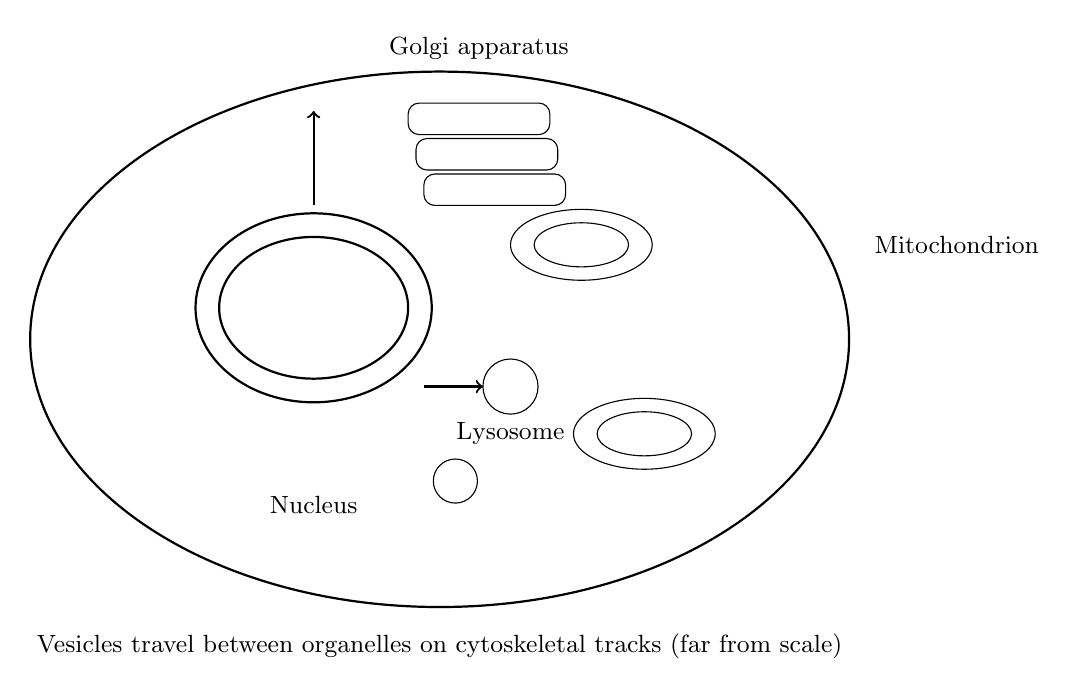
\begin{tikzpicture}[scale=1.0]
\draw[thick] (0,0) ellipse (5.2 and 3.4);
\draw[thick] (-1.6,0.4) ellipse (1.5 and 1.2);
\draw[thick] (-1.6,0.4) ellipse (1.2 and 0.9);
\draw (1.8,1.2) ellipse (0.9 and 0.45);
\draw (1.8,1.2) ellipse (0.6 and 0.28);
\draw (2.6,-1.2) ellipse (0.9 and 0.45);
\draw (2.6,-1.2) ellipse (0.6 and 0.28);
\draw[rounded corners=4pt] (-0.2,1.7) rectangle (1.6,2.1);
\draw[rounded corners=4pt] (-0.3,2.15) rectangle (1.5,2.55);
\draw[rounded corners=4pt] (-0.4,2.6) rectangle (1.4,3.0);
\draw (0.9,-0.6) circle (0.35);
\draw (0.2,-1.8) circle (0.28);
\draw[->,thick] (-1.6,1.7) -- (-1.6,2.9);
\draw[->,thick] (-0.2,-0.6) -- (0.55,-0.6);
\node at (-1.6,-2.1) {\small Nucleus};
\node[anchor=west] at (5.4,1.2) {\small Mitochondrion};
\node at (0.5,3.7) {\small Golgi apparatus};
\node at (0.9,-1.2) {\small Lysosome};
\node at (0,-3.9) {\small Vesicles travel between organelles on cytoskeletal tracks (far from scale)};
\end{tikzpicture}
\end{center}

\begin{table}[htbp]
\centering
\caption{Main eukaryotic organelles at a glance (plant-specific: chloroplasts, large vacuoles, cell walls)}
\begin{tabular}{lll}
\toprule
Organelle & Structure & Core mechanism \\
\midrule
Nucleus & \shortstack[l]{Double envelope\\with nuclear pores} & \shortstack[l]{DNA vault; pore proteins\\select what passes} \\
ER & Folded membrane maze & \shortstack[l]{Large working area; protein\\folding and lipid synthesis} \\
Golgi apparatus & Stacked membrane sacs & \shortstack[l]{Sugar-chain labels; vesicles\\deliver to addresses} \\
Lysosome & Single-membrane sac & \shortstack[l]{Proton pumps acidify interior;\\hydrolases work only in acid} \\
Mitochondrion & \shortstack[l]{Double envelope;\\inner cristae} & \shortstack[l]{Respiratory chain and\\ATP synthase (Chapter 53)} \\
Chloroplast & \shortstack[l]{Double envelope\\and thylakoids} & Photosynthetic chain (Chapter 54) \\
Cytoskeleton & \shortstack[l]{Microtubules and\\microfilaments} & \shortstack[l]{Assembled tracks and motors\\for directed transport} \\
\bottomrule
\end{tabular}
\end{table}

\section{Evidence: Ancient Tenants Inside Cells}

\begin{zhengju}
As early as the 1880s, microscopists noticed chloroplasts' striking resemblance to photosynthetic cyanobacteria. In 1905, the Russian scholar Mereschkowsky proposed that chloroplasts arose from swallowed bacteria that escaped digestion. The idea was bold, but without DNA sequences nobody could prove it, and it remained sidelined for over half a century.

In 1967, the American biologist Lynn Margulis submitted a paper developing the \textbf{endosymbiotic theory}: mitochondria and chloroplasts originated as engulfed bacteria. More than a dozen journals rejected it as unsupported and fanciful. She persisted in publishing, then waited with the wider biological community for over a decade for molecular biology's new tools. Evidence accumulated, each piece pointing to bacterial identity papers:

\begin{itemize}[itemsep=2pt]
\item \textbf{DNA:} mitochondria and chloroplasts contain their own circular DNA, like bacteria. Sequence comparison, whose principles appear from Chapter 66 onward, supplied the decisive blow. Mitochondrial sequences most closely resemble $\alpha$-proteobacteria, while chloroplast sequences point clearly to cyanobacteria. Membranes simply grown by a cell would have no obvious reason to carry bacterial-style hereditary material.
\item \textbf{Membranes:} both have double envelopes. Inner-membrane lipids resemble bacterial cell membranes, while outer ones resemble host food-engulfing vesicles. One engulfment without digestion neatly explains membranes from two origins. They also divide like bacteria, and cells cannot make new ones from nothing.
\item \textbf{Ribosomes:} their ribosomes are bacterial models, inhibited by certain antibiotics targeting bacterial ribosomes, while cytoplasmic ribosomes in the same cell are insensitive. Two protein-making machine types in one house require related but separate origins.
\end{itemize}

Alternatives were tested seriously: could these similarities be coincidence or genes moved in from the nucleus? Sequence evidence rejected them. The likeness was not superficial but letter by letter. Scientists can now even observe endosymbiosis in progress, with recently recruited cyanobacteria inside some single-celled organisms, halfway from tenant to organelle. The lesson is not merely Margulis's foresight, but that a repeatedly rejected theory can prevail through testable predictions. Incidentally, your mitochondrial DNA comes entirely from your mother's egg; paternal sperm mitochondria are cleared after fertilization, foreshadowing Volume III's inheritance story.
\end{zhengju}

\begin{shiyan}
\textbf{Watch Cells Working in Your Bowl} (safe to do at home)

Materials: a small packet of supermarket dry yeast, white sugar, warm water around $35\,^{\circ}\mathrm{C}$ and not hot to the touch, two transparent bottles, and two balloons.

Procedure: half-fill both bottles with warm water and add a spoonful of sugar to each. Add half a spoonful of dry yeast to one only and shake. Fit a balloon over each opening, leave somewhere warm, and observe after half an hour to an hour.

Observations: the yeast bottle's balloon gradually inflates while fine bubbles rise; the other remains inactive. The balloon gas is mainly \chem{CO_2}: yeast cells use Chapter 52's glycolysis to dismantle sugar and release gas along the way. You cannot see inside the cells, but their changing the bottle's chemistry is macroscopic evidence that cells are not empty bags.

Safety: only food-grade, nontoxic materials are used. Do not use hot water, which kills yeast and spoils the comparison. Pour the finished liquid down the sink and rinse away.

\textbf{Translator safety note:} Food ingredients do not make experimental mixtures safe to drink. Use plastic bottles with flexible balloons, never rigidly sealed containers; keep balloons away from young children, do not taste the liquid, and clean utensils afterward. These precautions apply the \href{https://www.acs.org/education/celebrating-chemistry-editions/2024-ccew/science-safety-tips.html}{ACS activity-safety guidance} to this gas-producing demonstration.
\end{shiyan}

\section{Where This Model Falls Short}

First, textbook organelle maps are frozen snapshots. Real mitochondria are not separate little sausages but a network constantly fusing, dividing, and rebuilding, changing topology within seconds. The ER is continuous; the Golgi disassembles and rebuilds during cell division. Treating organelles as fixed parts is the model's commonest misuse.

Second, simple prokaryotic structure does not mean uniform soup. Bacterial DNA has defined folding and locations, and cytoskeletal proteins related to eukaryotic ones follow geometrical arrangements to maintain rod shapes. Their organization simply does not rely on membrane compartments.

Third, eukaryotes with nuclei versus prokaryotes without is useful for known organisms, but the boundary is loosening. Some archaea from deep-sea sediments have many genes once thought exclusively eukaryotic and may be relatives of the ancient host. The host's identity and order of engulfment events remain disputed and revised: science is still alive here.

\begin{wuqu}
``Plant cells have chloroplasts, so they need no mitochondria.'' This mistakes photosynthesis and respiration for mutually exclusive alternatives. Chloroplasts work only in light and green tissues, converting light into sugar's chemical energy. Every living plant cell, including roots that never see light and leaves at night, needs mitochondria to turn sugar energy into immediately usable ATP, as in Chapter 53. A germinating underground seed has no green leaf and relies entirely on mitochondria. Put a houseplant in darkness for several days: it does not immediately die because mitochondria keep working. Without mitochondria, however, a plant cell could not survive a moment.
\end{wuqu}

\section{Back to the Yolk}

Now check your answer. The spilled yolk is less cell fluid than a huge \emph{supply warehouse}. Most of its volume is stored yolk proteins and lipids, provisions for a future embryo's twenty-one days. The truly crowded, active cytoplasm full of tracks and motors is a small white spot a few millimeters across on the surface, the germinal disc. All division, differentiation, and construction of the chick occur in that spot and its margins.

Why this arrangement? The diffusion calculation answers: crossing a three-centimeter cell by diffusion takes half a year, far too long. The egg's evolutionary strategy is a large warehouse and small factory. Even one of the world's largest cells rejects the bag-of-liquid picture. The bag holds supplies, not soup; its working corner is crowded and noisy, with railways, motors, and ancient tenants resident for billions of years.

\section{Going Deeper: Railway Drugs and Incoming Messages}

Understanding cytoskeletons explains one anticancer drug. Paclitaxel was first isolated from yew bark and disrupts microtubules' assembly--disassembly balance, freezing the tracks. Dividing cells use microtubules to move chromosomes, so rapidly dividing cancer cells stall and die. Normal cells are affected too, causing chemotherapy side effects. Chapter 59 returns to cancer from the perspective of cellular cooperation.

But we have skipped a more basic question: who schedules ER orders, Golgi shipments, lysosomal acidification, and motor departures? How does a cell know nutrients, danger, or neighbors' signals have arrived? Membrane antennas and signaling chains amplify a single external molecular message into a massive internal response. In Chapter 58, we explore how cells hear the outside world.

\begin{tiaozhan}
Why is diffusion slow? Imagine random molecular steps as coin tosses, each choosing a direction. Mathematics shows that after $N$ steps, mean-square distance from the origin is proportional to $N$, so distance scales with the square root of step count. In continuous form, $\langle x^2\rangle = 6Dt$ in three dimensions, making time $t$ proportional to distance \emph{squared}. This underlies the bridge calculation and explains why square roots recur in heat, Brownian motion, and even stock fluctuations. Geometry gives another estimate: cell volume and food demand grow with diameter cubed, while membrane area and intake capacity grow only with diameter squared. Doubling cell diameter increases the volume each organelle must feed eightfold. This cube-versus-square race is a geometric reason cells cannot grow indefinitely and eggs need special arrangements. Skipping this box does not affect the main argument.
\end{tiaozhan}

\section*{Practice}

\begin{sikaoti}
\item Draw a protein-delivery map from a ribosome through ER, vesicle, Golgi, vesicle, and cell membrane for a membrane protein. Beside each station, write a sentence describing what its molecules do.
\item Using the bridge method, estimate diffusion time across a \ud{10}{\mu m} nucleus with $D\approx\ud{10}{\mu m^2/s}$, then along a meter-long nerve-cell axon. Explain why axons need molecular motors.
\item List the three kinds of endosymbiosis evidence given here: DNA, membranes, and ribosomes. For each, state what would be expected if mitochondria were membranes made by the cell itself, and what is actually observed.
\item Lysosomes combine an acidic interior with enzymes that work efficiently only in acid. Using Chapter 34's $pH$--enzyme relationship, sketch a possible hydrolase-activity curve against $pH$ and mark the lysosomal and cytoplasmic operating points.
\item A prokaryote has no mitochondria but must make ATP. Use Chapter 53's account of the respiratory chain in membranes to suggest where a bacterial chain would be located. Does this support the endosymbiotic account of mitochondrial inner membranes?
\end{sikaoti}
